\pdfoutput=1

\documentclass[11pt]{article}

\usepackage[]{acl}

\usepackage{times}
\usepackage{latexsym}
\usepackage{bm}


\usepackage[T1]{fontenc}

\usepackage[utf8]{inputenc}

\usepackage{microtype}

\usepackage{algorithm}
\usepackage{algorithmic}
\usepackage{url}            \usepackage{booktabs}       \usepackage{amsfonts}       \usepackage{nicefrac}       \usepackage{microtype}      \usepackage{xcolor}         \usepackage{lipsum}
\usepackage{arydshln}
\usepackage{pgfplots}
\usepackage[encapsulated]{CJK}
\usepackage{multirow}
\usepackage{mathrsfs}
\usepackage{mathtools}
\usepackage{subfigure}
\pgfplotsset{compat=1.15}
\hyphenpenalty=8000
\usepackage[draft]{changes}

\title{Document-Level Relation Extraction with Sentences Importance Estimation and Focusing}

\author{Wang Xu\textsuperscript{\rm 1}, Kehai Chen\textsuperscript{\rm 1}, Lili Mou\textsuperscript{\rm 2}, Tiejun Zhao\textsuperscript{\rm 1} \\
  \textsuperscript{\rm 1}Harbin Institute of Technology, China \\
  \textsuperscript{\rm 2}Dept. Computing Science, Alberta Machine Intelligence Institute (Amii)\\
  University of Alberta, Canada \\
  xuwang@hit-mtlab.net, \{chenkehai,tjzhao\}@hit.edu.cn, doublepower.mou@gmail.com\\}


\begin{document}
\maketitle
\begin{abstract}
Document-level relation extraction~(DocRE) aims to determine the relation between two entities from a document of multiple sentences.
Recent studies typically represent the entire document by sequence- or graph-based models to predict the relations of all entity pairs. However, we find that such a model is not robust and exhibits bizarre behaviors: it predicts correctly when an entire test document is fed as input, but errs when non-evidence sentences are removed. To this end, we propose a Sentence Importance Estimation and Focusing (SIEF) framework for DocRE, where we design a sentence importance score and a sentence focusing loss, encouraging DocRE models to focus on evidence sentences. Experimental results on two domains show that our SIEF not only improves overall performance, but also makes DocRE models more robust. Moreover, SIEF is a general framework, shown to be effective when combined with a variety of base DocRE models.\footnote{The code is publicly available at \url{https://github.com/xwjim/SIEF}}
\end{abstract}

\section{Introduction}
\label{sec1}

Document-level relation extraction (DocRE) aims to predict entity relations across multiple sentences. It plays a crucial role in a variety of knowledge-based applications, such as question answering~\cite{sorokin-gurevych-2017-context} and large-scale knowledge graph construction~\cite{baldini-soares-etal-2019-matching}.
Different from sentence-level relation extraction~\cite{zeng-etal-2014-relation,xiao-liu-2016-semantic,Song_2019}, the supporting evidence in the DocRE setting may involve multiple sentences scattering in the document. 
Thus, DocRE is more a realistic setting, attracting increasing attention in the field of information extraction.

\begin{figure}[t!]
  \centering
  \includegraphics{example.pdf}
  \caption{A DocRE model predicts correctly for an entire document, but errs when a non-evidence sentence is removed.}
  \label{fig1:example}
\end{figure}


Most recent DocRE studies use the entire document as a clue to predict the relations of all entity pairs without concerning where the evidence is located~\cite{Nan2020ReasoningWL,zeng-etal-2020-double,xu-etal-2021-discriminative,docred-rec}. 
However, one can identify the relation of a specific entity pair from a few sentences.
\citet{huang-etal-2021-three} show that irrelevant sentences in the document would hinder the performance of the model. 

Moreover, we observe that a DocRE model, trained on the entire document, may err when non-evidence sentences are removed.
In Figure~\ref{fig1:example}, for example, we need to identify the relation ``MemberOf'' between the entities \textit{Brad Wilk} and \textit{Rage Against the Machine}.
The evidence sentences are \{1,2\}, and humans can easily identify such a relation when reading sentences \{1,2\} only.
However, the recent DocRE model GAIN~\cite{zeng-etal-2020-double} identifies the relation ``MemberOf'' correctly from the entire document \{1,2,3\}, but predicts ``not MemberOf'' from sentences \{1,2\}. 
Intuitively, removing sentence \{3\} should not change the result, as this sentence does not provide information regarding whether ``MemberOf'' holds or not for the two entities.
Such model behaviors are undesired, because it shows that the model is not robust and lacks interpretability. 

To this end, we propose a novel \textbf{S}entence \text{I}mportance \textbf{E}stimation and \textbf{F}ocusing~(\textbf{SIEF}) framework to encourage the model to focus on evidence sentences for predicting the relation of an entity pair.
Specifically, we first evaluate the importance of each sentence by the difference between the output probabilities of the document with and without this sentence. If the predicted probability of a relation does not change, or even increases, when a sentence is removed, it typically indicates that the sentence is \textit{non-evidence}.
Then, we propose an auxiliary loss to encourage the model to produce the same output distribution, when the entire document is fed as input and when a non-evidence sentence is removed.
In this way, the model pays more attention to the evidence sentences for the classification.
Our SIEF method is a general framework that can be combined with different underlying DocRE models.

We evaluated the generality and effectiveness of our approach on the large-scale DocRED dataset~\cite{yao-etal-2019-docred}.
Experimental results show that the proposed approach combines well with various recent DocRE models and significantly improves the performance.
We further evaluated our approach on a dialogue relation extraction dataset, DialogRE~\cite{yu-etal-2020-dialogue}; our SIEF yields consistent improvement, showing the generality of our approach in different domains.

\section{Related Work}
\label{sec2}
Relation extraction (RE) can be categorized by its granularity, such as sentence-level~\cite{doddington-etal-2004-automatic,xu-etal-2016-improved,wei2019novel} and document-level~\cite{DBLP:journals/corr/abs-1810-05102,zhu-etal-2019-graph}.
Early work mainly focuses on sentence-level relation extraction. \newcite{pantel-pennacchiotti-2006-espresso} propose a rule-based approach, and \newcite{mintz-etal-2009-distant} manually design features for classifying relations. In the past several years, neural networks have become a prevailing approach for relation extraction~\cite{xu-etal-2015-classifying,Song_2019}.

Document-level relation extraction~(DocRE) is attracting increasing attention in the community, as it considers the interactions of entity mentions expressed in different sentences~\cite{Li2016cdr,yao-etal-2019-docred}. Compared with the sentence level, DocRE requires the model collecting and integrating inter-sentence information effectively. Recent efforts design sequence-based and graph-based models to address such a problem.

Sequence-based DocRE models encode a document by the sequence of words and/or sentences, for example, using the Transformer architecture~\cite{devlin-etal-2019-bert}.
\newcite{zhou2021atlop} argue that the Transformer attentions are able to extract useful contextual features across sentences for DocRE, and they adopt an adaptive threshold for each entity pair.
\newcite{ijcai2021-551} model DocRE as a semantic segmentation task and predict an entity-level relation matrix to capture local and global information.

Graph-based DocRE models abstract a document by graphical structures. For example, a node can be a sentence, a mention, and/or an entity; their co-occurrence is modeled by an edge. Then graph neural networks are applied to aggregate inter-sentence information~\cite{quirk-poon-2017-distant,Christopoulou2019ConnectingTD,zeng-etal-2020-double}. 
\newcite{zeng-etal-2020-double} construct double graphs, applying graph neural networks to mention--document graphs and performing path reasoning over entity graphs.
\newcite{xu-etal-2021-discriminative} explicitly incorporate logical reasoning, common-sense reasoning, and coreference reasoning into DocRE, based on both sequence and graph features.

Different from previous work, our paper proposes SIEF as a general framework that can be combined with various sequence-based and graph-based DocRE models. In our approach, we propose a sentence importance score and a sentence focusing loss to encourage the model to focus on evidence sentences, improving the robustness and the overall performance of DocRE models.

\begin{figure*}[ht!]
  \centering
  \includegraphics{data_consist.pdf}
  \caption{We estimate the sentence importance (for a specific entity pair and relation) by the difference of the classification probabilities with and without the sentence. Then, we encourage the DocRE model to predict the same probability when the entire document is fed as input and when a non-evidence sentence is removed.}
  \label{fig2:data_consistent}
\end{figure*}

\section{Problem Definition}
\label{sec3}
In this section, we present the formulation of document relation extraction (DocRE). Consider an unstructured document comprising  sentences, , where each sentence  is a sequence words. In a DocRE dataset, the document  is typically annotated with entity mentions, each mention (e.g., U.S.~and USA) labeled by its conceptual entity  and its entity type (e.g., location).

A DocRE model  is usually formulated as multi-label classification~\cite{yao-etal-2019-docred}.  predicts  whether the th relation holds for the th marked entity pair in a document, given by

where  is the head entity and  is the tail entity;   is the groundtruth label regarding entity pair  and relation .

To train the model, the binary cross-entropy loss is used as the objective for parameter estimation:

where  denotes the entire corpus and  denotes the set of relation types.

During inference, we obtain the relation(s) of a given entity pair by thresholding the predicted probabilities, following most previous work~\cite{yao-etal-2019-docred,zhou2021atlop}.

\section{Methodology}
\label{sec4}

In this section, we will describe our approach in detail.
The overview of our framework is shown in Figure~\ref{fig2:data_consistent}.
First, we describe the estimation of sentence importance in Section \ref{sec4-1}.
Sentences with low importance scores are treated as non-evidence.
Then, Sections~\ref{sec4-2} and \ref{sec4-3} present our approach that encourages the model to produce the same output distribution, when the entire document is fed as input and when  non-evidence sentences are removed.
 Section~\ref{sec4-4} further presents the architectures of DocRE models.

\subsection{Sentence Importance Estimation}
\label{sec4-1}
We estimate the importance of each sentence for a specific entity pair. Low-scored sentences will be treated as non-evidence, and in principle, can be removed without changing DocRE predictions. 

We propose a sentence importance score based on the DocRE predictions with and without the sentence in question. 
Our observation is that the relation extraction task is usually monotonic to evidence, i.e., (non-strictly) more relations will be predicted with more sentences. 
If we remove a sentence and the predicted probability of a relation decreases, then the sentence is likely to be the evidence.
If the predicted probability does not change, then the sentence is likely to be non-evidence. Moreover, the predicted probability may sometimes increase when a sentence is removed, in which case the DocRE model is not robust, as this violates monotonicity.

Formally, we consider removing one sentence at a time, and the document with the th sentence removed is denoted by .
For a DocRE model , we obtain the classification probabilities  based on the original document, and  with sentence  removed.

We propose the importance score as 


The formula appears similar to Kullback--Leibler (KL) divergence. 
However, we only take one term in the KL summation, because the KL divergence, albeit asymmetric in its two arguments, cannot model the increase or decrease of , whereas our  is monotonically decreasing with . 
Compared with a naive difference or ratio between  and , we find that our KL-like score is more robust in the scale of  when determining non-evidence sentences.

We treat a sentence  as \textit{non-evidence} if  for a thresholding hyperparameter .
The resulting set of non-evidence sentences is denoted by  for the an entity pair  and relation~.

\subsection{Sentence Focusing Loss}
\label{sec4-2}
We propose a sentence focusing loss to encourage the model to produce the same output distribution when the entire document is fed as input and when non-evidence sentences are removed.

Ideally, the predicted probability should remain the same if we remove any combination of the sentences in . Therefore, we penalize the extent to which the predicted probability is changed.

We propose the sentence focusing loss as:

where  is a subset of  and  is the predicted probability with  removed from , and the total loss is .

Essentially, our sentence focusing loss ensures  is close to , which intuitively makes sense because non-evidence sentences should not affect the prediction. Our approach can also be thought of as a way of data augmentation.
However, compared with one-hot groundtruth labels, our sentence focusing loss works with soft labels  and , which are believed to contain more information~\cite{kd44873}, and our gradient propagates to both  and  for training. 

The calculation of Eqn.~\eqref{eq4} is time- and resource-consuming, because the number of the subsets  grows combinatorially with the number of non-evidence sentences. 
Moreover it should be calculated repeatedly once the parameter of the model is updated.
To this end, we propose a simplified training strategy to approximate Eqn.~\eqref{eq4} in the next subsection.

\subsection{Training Strategy}
\label{sec4-3}
We propose a strategy to simplify the calculation and the training procedure.
Concretely, we only remove one non-evidence sentence in  at a time instead of a subset of , and we aggregate the effect of different non-evidence sentences by:

where  is the indicator function. Essentially, we linearly approximate the combination of multiple non-evidence sentences in \eqref{eq4}  by an outer summation. In this way, the number of terms does not grow combinatorially, but linearly w.r.t.~.

In implementation, we further simply the summation over  by Monte Carlo sampling of a randomly selected sentence~ in each gradient update.
The loss is reformulated as follows:


As seen, we need to forward the base models twice in each update, with and without the sentence . 
\citet{huang-etal-2021-three} propose a similar idea but train different entity pairs in a document based on different sets of sentences; all sentence are processed repeatedly among entity pairs in a document. Their approach is much slower than ours.

To sum up, the proposed SIEF framework identifies non-evidence sentences and penalizes the difference of predicted probabilities when a non-evidence sentence is removed. 
Our approach is a generic framework and can be adapted to various DocRE model easily, without introducing extra parameters into the model.

\subsection{DocRE Model Architectures}
\label{sec4-4}
Our SIEF can be applied to various base DocRE models.
To evaluate its generality, we consider the following recent models. 

\textbf{BiLSTM}~\cite{yao-etal-2019-docred}\footnote{https://github.com/thunlp/DocRED\label{rep_docred}}. A bi-directional long short term memory (BiLSTM) encodes the document, and an entity is representated by BiLSTM's hidden states, averaged over entity mentions. The head and tail entity representations are fed to a multi-layer perceptron (MLP) for relation extraction.

\textbf{BERT}~\cite{devlin-etal-2019-bert}\footnote{https://github.com/DreamInvoker/GAIN\label{rep_gain}}. A pre-trained language model is used for document encoding.

\textbf{HeterGSAN}~\cite{docred-rec}\footnote{https://github.com/xwjim/DocRE-Rec\label{rep_rec}}. HeterGSAN is a recent graph-based DocRED model, which constructs a heterogeneous graph of sentence, mention, and entity nodes; it uses graph neural networks for relation extraction.

\textbf{GAIN}~\cite{zeng-etal-2020-double}\textsuperscript{\ref {rep_gain}}. GAIN constructs two graphs: mention--document graphs and entity graphs, and performs graph and path reasoning over the two graphs separately. When combining our SIEF with GAIN, we achieve the best performance among all the base models with SIEF on DocRED. Thus, we will explain this model in more detail.

Essentially, a node in the mention--document graph is either a mention or a document. The mentions are connected to its document, and two mentions are connected if they co-occur in one sentence. In the entity graph, two entities are connected if they are mentioned in one sentence. To classify the relation, GNN is applied to the mention--document graph, enhanced with path information in the entity graph, shown in Figure~\ref{fig3:model_arch}.

\begin{figure}[!t]
  \centering
  \includegraphics{model_arch.pdf}\vspace{-.2cm}
  \caption{The model architecture of GAIN with SIEF. A sentence is randomly removed from the document. The corresponding nodes and edges are removed from the mention--document graph and the entity graph.}\vspace{-.2cm}
  \label{fig3:model_arch}
\end{figure}

When combining SIEF with GAIN, we randomly remove one sentence from the document. The corresponding nodes and edges are removed in the GAIN's graphs.
Then we obtain the output probabilities with and without the sentence,  and , separately.
If the sentence important score  in Eqn.~\eqref{eq3} is below a threshold , the sentence is treated as non-evidence for the entity pair  and relation . We apply the sentence focusing loss Eqn.~\eqref{eq4} to improve the robustness.

For prediction, we apply the trained DocRE model to the entire document, because with our approach the model is already robust when non-evidence sentences are presented. Empirical results will show that our SIEF consistently improves the performance of base DocRE models. 

\section{Experiments}
\label{sec5}
\subsection{Setup}
\label{sec5-1}
\noindent \textbf{Datasets.} DocRED is a large-scale human-annotated dataset for document-level relation extraction~\cite{yao-etal-2019-docred}.
The dataset is constructed from Wikipedia and Wikidata, containing 3053 documents for training, 1000 for development, and 1000 for test. In total, it has 132,375 entities and 56,354 relational facts in 96 relation types. 
More than 40\% of the relational facts require reasoning over multiple sentences.
The standard evaluation metrics are F1 and Ign~F1 \cite{yao-etal-2019-docred,zeng-etal-2020-double}, where Ign~F1 refers to the F1 score excluding the relational facts in the training set.

We also evaluated our approach on \mbox{DialogRE} \cite[V2,][]{yu-etal-2020-dialogue}, which contains 36 relation types, 17 of which are interpersonal. We followed the standard split with 1073 training dialogues, 358 validation, and 357 test. Following \newcite{yu-etal-2020-dialogue}, we report macro F1 scores in both the standard and conversational settings; the latter is denoted by F1.

\textbf{Competing Methods.} We experimented our SIEF on a number of base models, namely, BiLSTM, BERT, HeterGSAN, and GAIN (Section~\ref{sec4-4}). 
These base models are all considered for comparison. 

For DocRED, we consider additional competing methods: 
\textbf{Two Phase}~\cite{Wang2019FinetuneBF}, which first predicts whether the entity pair has a relation and then predicts the relation type;
\textbf{LSR}~\cite{Nan2020ReasoningWL}, which constructs the graph by inducing a latent document-level graph;
\textbf{Reconstructor}~\cite{docred-rec}, which encourages the model to reconstruct a reasoning path during training;
\textbf{DRN}~\cite{xu-etal-2021-discriminative}, which considers different reasoning skills explicitly and uses graph representation and context representation to model the reasoning skills;
\textbf{ATLOP}~\cite{zhou2021atlop}, which aggregates contextual information by the Transformer attentions and adopts an adaptive threshold for different entity pairs;
and \textbf{DocuNet}~\cite{ijcai2021-551}, which models DocRE as a semantic segmentation task.

For DialogRE, we followed \newcite{yu-etal-2020-dialogue} and considered \textbf{BERT} and \textbf{BERT} for comparison,\footnote{https://github.com/nlpdata/dialogre\label{rep_dialog}}
where \textbf{BERT} prevents a model from overfitting by replacing of the interpersonal augment with a special token.

\textbf{Implementation Details}. We use the repositories\textsuperscript{\ref {rep_docred},\ref{rep_gain},\ref{rep_rec},\ref{rep_dialog}} of base models to implement our approach.
We mostly followed the standard hyperparameters used in the base models. 
Our SIEF has one hyperparameter  in Eqn.~\eqref{eq6}. It was set to 0.8, and Section~\ref{sec5-2} presents the effect of tuning .

\subsection{Results and Analyses}
\label{sec5-2}
\begin{table}[!t]
\begin{center}
\scalebox{.69}{
\begin{tabular}{l|l|l|l|l}
\hline \hline
\multicolumn{1}{c|}{\multirow{2}{*}{Model}} & \multicolumn{2}{c|}{Dev} & \multicolumn{2}{c}{Test} \\ \cline{2-5} 
                       \multicolumn{1}{c|}{}                       & Ign F1        & F1       & Ign F1        & F1        \\ \hline
\multicolumn{5}{c}{\textit{DocRE Systems with GloVe}}                                    \\ \hline
 LSR~\cite{Nan2020ReasoningWL}          & 48.82 & 55.17 & 52.15 & 54.18 \\ 
 Reconstructor~\cite{docred-rec}        & 54.25 & 55.70 & 53.25 & 55.13   \\  
 DRN~\cite{xu-etal-2021-discriminative} & 54.61 & 56.49 & 54.35 & 56.33     \\\hline
  BiLSTM~\cite{yao-etal-2019-docred}            & 48.87 & 50.94 & 48.78 & 51.06 \\
 \;\;\;+\textbf{SIEF}                 & 52.08 & 54.20 & 51.03 & 53.22 \\   \cdashline{1-5}
 HeterGSAN~\cite{docred-rec}            & 52.17 & 54.40 & 52.07 & 53.52\\
 \;\;\;+\textbf{SIEF}                 & 54.49 & 56.30 & 53.94 & 55.85\\  \cdashline{1-5}
 GAIN~\cite{zeng-etal-2020-double}      & 53.05 & 55.29 & 52.66 & 55.08 \\  
 \;\;\;+\textbf{SIEF}                 & 55.07 & 56.96 & 54.72 & 56.75\\  \hline \hline 
\multicolumn{5}{c}{\textit{DocRE Systems with BERT}}                                              \\ \cline{1-5} 
Two-Phase~\cite{Wang2019FinetuneBF}     & -     & 54.42 & -     & 53.92\\
LSR~\cite{Nan2020ReasoningWL}           & 52.43 & 59.00 & 56.97 & 59.05 \\ 
Reconstructor~\cite{docred-rec}     & 58.13 & 60.18 & 57.12 & 59.45 \\ 
DRN~\cite{xu-etal-2021-discriminative} & 59.33 & 61.39 & 59.15 & 61.37 \\
ATLOP~\cite{zhou2021atlop}     & 59.22 & 61.09 & 59.31 & 61.30 \\
DocuNet~\cite{ijcai2021-551} & 59.86 & 61.83 & {\textbf{59.93}} & 61.86  \\ \hline
BERT~\cite{ye-etal-2020-coreferential}          & 54.63 & 56.77 & 53.93 & 56.27 \\ 
\;\;\;+\textbf{SIEF}                 & 57.13 & 59.11 & 57.87 & 58.93\\  \cdashline{1-5}
HeterGSAN~\cite{docred-rec}         & 57.00 & 59.13 & 56.21 & 58.54 \\
\;\;\;+\textbf{SIEF}             & 57.99 & 60.04 & 57.93 & 60.02   \\  \cdashline{1-5}
GAIN~\cite{zeng-etal-2020-double}   & 59.14 & 61.22 & 59.00 & 61.24 \\ 
\;\;\;+\textbf{SIEF}             & \textbf{59.82} & \textbf{62.24} & {59.87} & \textbf{62.29}   \\ \hline \hline
\end{tabular}}
\end{center}
\caption{Results on the development and test sets of the DocRE dataset. 
Bold indicates the best performance.}
\label{tab:mainresult} 
\end{table}

\begin{table}[!t]
\centering
\resizebox{0.9\linewidth}{!}{
\begin{tabular}{l|cc|cc}
\hline
\multirow{2}{*}{Model} & \multicolumn{2}{c|}{Dev} & \multicolumn{2}{c}{Test} \\ \cline{2-5} 
                       & F1     & F1  & F1   & F1       \\ \hline
BERT~\cite{yu-etal-2020-dialogue}                   & 60.6   & 55.4    & 58.5 & 53.2          \\
\;\;\;+\textbf{SIEF}             & 61.4   & 57.6    & 59.9 & 56.1         \\ \hline
BERT~\cite{yu-etal-2020-dialogue}               & 63.0   & 57.3    & 61.2 & 55.4             \\
\;\;\;+\textbf{SIEF}             & \textbf{64.3}   & \textbf{60.6}  & \textbf{61.8} & \textbf{58.4}          \\ \hline
\end{tabular}}
\caption{Results on DialogRE.}
\label{tab:dialogre}
\end{table}

\textbf{Main results.}
Table~\ref{tab:mainresult} presents the detailed results on the development and test sets of the DocRED dataset. 
We first compare DocRE systems with GloVe embeddings~\cite{yao-etal-2019-docred}. We see that the proposed SIEF method significantly improves the performance of all base models, including the sequence model (i.e., BiLSTM) and graph models (i.e., HeterGSAN and GAIN); the average improvement is 2.05 points in terms of test F1. This shows that SIEF is compatible with both sequence and graph models, indicating the generality and effectiveness of the proposed method.

For the DocRE system with BERT, SIEF also consistently improves the base models, showing that SIEF is complementary to the modern BERT architecture. Especially, combining SIEF and GAIN~\cite{zeng-etal-2020-double} with BERT encoding yields state-of-the-art performance in terms of F1.

We further conducted experiments on the DialogRE dataset, and compare our approach with the BERT baselines in \newcite{yu-etal-2020-dialogue}. As seen, the results are consistent with the improvement on DocRED, as our SIEF largely improves F1 and F1 for both base models. This further confirms the generality of our approach in different domains.

In the rest of this section, we present in-depth analyses to better understand our model with DocRED as the testbed. All base models use GloVe embeddings as opposed to BERT due to efficiency concerns.
\begin{figure*}[ht!]\centering
\resizebox{.8\linewidth}{!}{
    \begin{minipage}[b]{0.32\linewidth}
    \centering
		\pgfplotsset{height=4.5cm,width=6.0cm,compat=1.14,every axis/.append style={thick},every axis legend/.append style={at={(1,0.13)}},legend columns=1}
		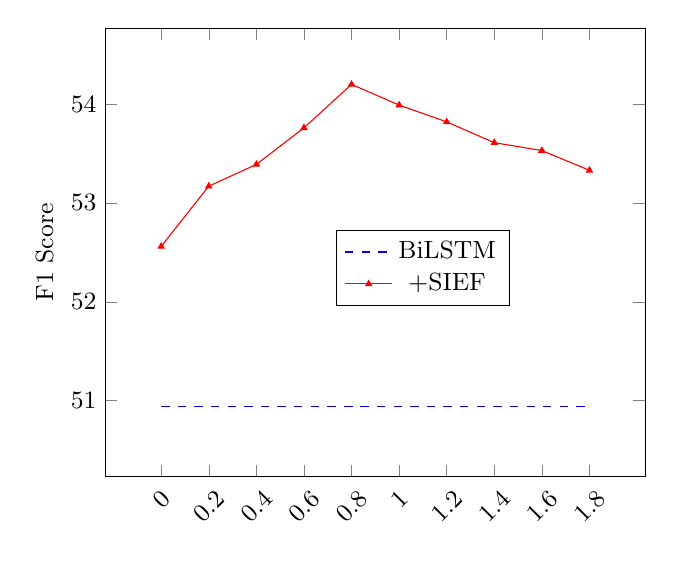
\begin{tikzpicture}
		\tikzset{every node}=[font=\small]
		\begin{axis}
		[enlargelimits=0.13, tick align=inside, 
		xtick={0,0.2,0.4,0.6,0.8,1.0,1.2,1.4,1.6,1.8},
		x tick label style={rotate=45},
		ymin=50.7,
		ymax=54.3,
		legend style={at={(0.75,0.55)}},
		ylabel={F1 Score},xlabel={},font=\small]
		\addplot [dashed,mark size=1.2pt,mark options={solid,mark color=blue}, color=blue] coordinates
		{(0,50.94)(0.2,50.94)(0.4,50.94)(0.6,50.94)(0.8,50.94)(1.0,50.94)(1.2,50.94)(1.4,50.94)(1.6,50.94)(1.8,50.94)};
		\addlegendentry{\small BiLSTM}
		\addplot [sharp plot,mark=triangle*,mark size=1.2pt,mark options={solid,mark color=red}, color=red] coordinates
		{(0,52.56)(0.2,53.17)(0.4,53.39)(0.6,53.76)(0.8,54.20)(1.0,53.99)(1.2,53.82)(1.4,53.61)(1.6,53.53)(1.8,53.33)};
		\addlegendentry{\small +SIEF}
		\end{axis}
		\end{tikzpicture}
		    \end{minipage}
    \hspace{0.5cm}
        \begin{minipage}[b]{0.32\linewidth}
    \centering
    \pgfplotsset{height=4.5cm,width=6.0cm,compat=1.14,every axis/.append style={thick},every axis legend/.append style={at={(1,0.13)}},legend columns=1}
		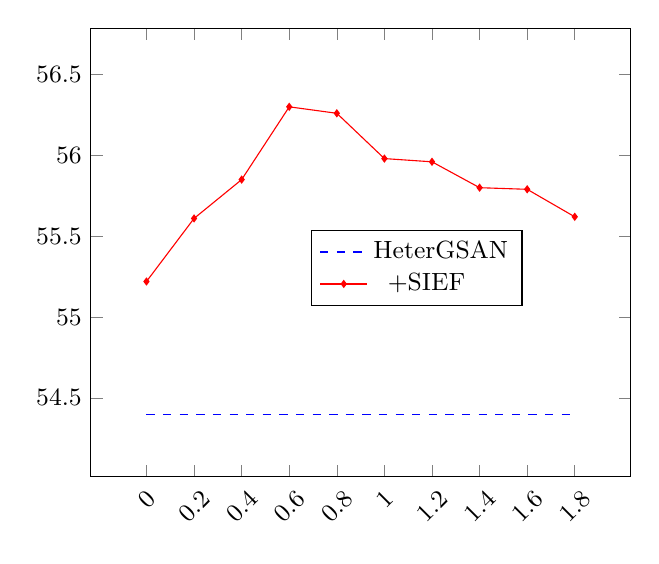
\begin{tikzpicture}
		\tikzset{every node}=[font=\small]
		\begin{axis}
		[enlargelimits=0.13, tick align=inside, 
		xtick={0,0.2,0.4,0.6,0.8,1.0,1.2,1.4,1.6,1.8},
		x tick label style={rotate=45},
		ymin=54.3,
		ymax=56.5,
		legend style={at={(0.80,0.55)}},
		xlabel={},font=\small]
		\addplot [dashed,mark size=1.2pt,mark options={solid,mark color=blue}, color=blue] coordinates
		{(0,54.40)(0.2,54.40)(0.4,54.40)(0.6,54.40)(0.8,54.40)(1.0,54.40)(1.2,54.40)(1.4,54.40)(1.6,54.40)(1.8,54.40)};
		\addlegendentry{\small HeterGSAN}
		\addplot [sharp plot,mark=diamond*,mark size=1.2pt,mark options={solid,mark color=red}, color=red] coordinates
		{(0,55.22)(0.2,55.61)(0.4,55.85)(0.6,56.30)(0.8,56.26)(1.0,55.98)(1.2,55.96)(1.4,55.80)(1.6,55.79)(1.8,55.62)};
		\addlegendentry{\small +SIEF\;\;\;\;}
		\end{axis}
		\end{tikzpicture}
		\end{minipage}
    \hspace{0.35cm}
    \begin{minipage}[b]{0.32\linewidth}
    \centering
    \pgfplotsset{height=4.5cm,width=6.0cm,compat=1.14,every axis/.append style={thick},every axis legend/.append style={at={(1,0.13)}},legend columns=1}
		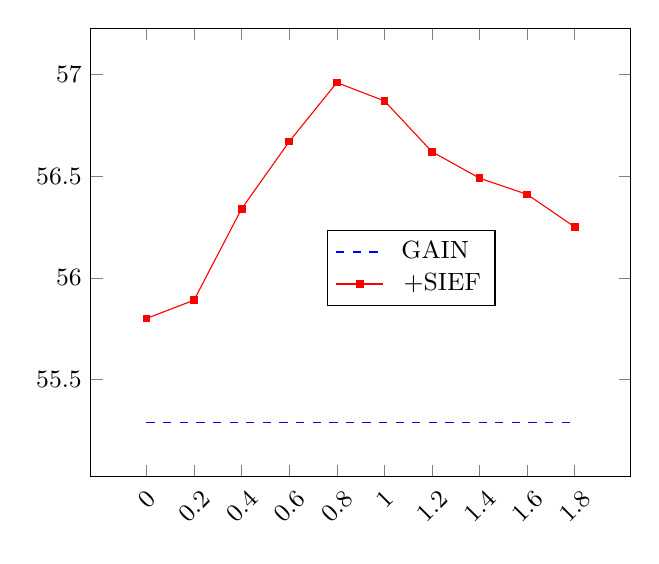
\begin{tikzpicture}
		\tikzset{every node}=[font=\small]
		\begin{axis}
		[enlargelimits=0.13, tick align=inside, 
		xtick={0,0.2,0.4,0.6,0.8,1.0,1.2,1.4,1.6,1.8},
		x tick label style={rotate=45},
		ymin=55.25,
		ymax=57.0,
		legend style={at={(0.75,0.55)}},
		xlabel={},font=\small]
		\addplot [dashed,mark size=1.2pt,mark options={solid,mark color=blue}, color=blue] coordinates
		{(0,55.29)(0.2,55.29)(0.4,55.29)(0.6,55.29)(0.8,55.29)(1.0,55.29)(1.2,55.29)(1.4,55.29)(1.6,55.29)(1.8,55.29)};
		\addlegendentry{\small GAIN}
		\addplot [sharp plot,mark=square*,mark size=1.2pt,mark options={solid,mark color=red}, color=red] coordinates
		{(0,55.80)(0.2,55.89)(0.4,56.34)(0.6,56.67)(0.8,56.96)(1.0,56.87)(1.2,56.62)(1.4,56.49)(1.6,56.41)(1.8,56.25)};
		\addlegendentry{\small \;\;+SIEF}
		\end{axis}
		\end{tikzpicture}
		\end{minipage}}\vspace{-.35cm}
		\caption{\label{fig:hypertheta}Performances of the classification (in F1 scores) on the development set of different hyperparameter  in Eqn.~\eqref{eq7} during the training.}\vspace{-.2cm}
\end{figure*}

\textbf{Intra- and Inter-Sentence Performance.}
We breakdown the relation classification performance into intra-sentence reasoning and inter-sentence reasoning. Ideally, if only one sentence is needed to determine the relation of an entity pair, then it belongs to the intra-sentence category; if two or more sentences are needed, then it belongs to the inter-sentence category. We follow~\newcite{Nan2020ReasoningWL} and approximate it by checking whether two entities are mentioned in one sentence.

The results are shown in Table~\ref{tab:reasonperformance}. SIEF again consistently improves base models in terms of both Intra-F1 and Inter-F1. However, the improvement on Intra-F1 is larger than that on Inter-F1. This is because our SIEF encourages the model to focus on evidence by removing one sentence at a time, but does not explicitly model sentence relations. Based on this analysis, we plan to extend the SIEF framework with multi-sentence DocRE reasoning in our future work.

\begin{table}[!t]
\centering
\resizebox{0.8\linewidth}{!}{
\begin{tabular}{l|ll}
\hline
Model             & Intra-F1     & Inter-F1    \\ \hline
BiLSTM            & 57.05 & 43.49   \\
\;\;\;\;+\textbf{SIEF}      & 60.56  & 45.96   \\ \hline
HeterGSAN         & 61.79 & 47.06   \\
\;\;\;\;+\textbf{SIEF}      & 63.01  & 48.11   \\ \hline
GAIN              & 61.67 & 48.77   \\
\;\;\;\;\textbf{+SIEF}      & \textbf{63.21}  & \textbf{48.98}   \\ \hline
\end{tabular}}
\caption{Results of Intra-F1 results and Infer-F1 on development set of DocRED. The difference is compared between SIEF and the respective base model.}
\label{tab:reasonperformance}
\end{table}


\textbf{Performance of predicting evidence sentences.} 
In our paper, we propose a sentence importance score to measure how much a sentence contributes to the classification without using additional annotation. We evaluate such performance in Table~\ref{tab:performanceevidence} by Precision, Recall, and F1 scores against manually annotated evidence sentences that are provided in the dataset. In this analysis, we do not perform relation prediction, but concern about entity pairs knowingly having certain relations.
Specifically, for entity pair  with relation , we calculate the importance score  for each sentence and cut off evidence/non-evidence sentences with a threshold based on the development F1 score. 

As seen, all base models achieve above 60\% F1, suggesting that the proposed importance score is indeed indicative for predicting evidence and non-evidence sentences.

With the proposed SIEF framework, the performance improves for all metrics, with an average improvement of 2.95 F1 points across three base models.
This further verifies that our SIEF framework not only improves relation extraction performance, but also is able to better detect evidence and non-evidence sentences, which is important for the interpretability of machine learning models.


\begin{table}[!t]
\centering
\resizebox{0.8\linewidth}{!}{
\begin{tabular}{l|lll}
\hline
Model     & Precision   & Recall & F1    \\ \hline
BiLSTM            & 60.14 & 68.41  & 64.01 \\
\;\;\;\;+\textbf{SIEF}      & 65.00 & 67.99  & 66.46 \\ \hline
HeterGSAN         & 65.40 & 70.95  & 68.06 \\
\;\;\;\;+\textbf{SIEF}      & 71.40 & 70.21  & 70.80 \\ \hline
GAIN              & 65.28 & 71.17  & 68.10 \\
\;\;\;\;+\textbf{SIEF}      & \textbf{71.94} & \textbf{71.60}  & \textbf{71.77} \\ \hline
\end{tabular}}\vspace{-.1cm}
\caption{Results of the evidence prediction on the development set of DocRED.}\vspace{-.2cm}
\label{tab:performanceevidence}
\end{table}

\begin{figure}[!t]\vspace{-.3cm}
  \centering
  \includegraphics{only_node.jpg} \vspace{-.6cm}
  \caption{Robustness of DocRE models.}\vspace{-.2cm}
  \label{fig:data_point_dis}
\end{figure}

\textbf{Robustness of DocRE models.}
We further investigate the robustness of DocRE models by showing the difference between the predicted distributions with and without non-evidence sentences. We show  in Figure~\ref{fig:data_point_dis}  the scatter plots of the probability  based on the entire document and the probability  with a random non-evidence sentence removed. 

As shown in the figure, the points of the base models (left magenta plots) scatters over a wider range, whereas our SIEF training (right cyan plots) makes them more concentrated on the diagonal, indicating that the prediction  on the entire document is mostly the same as  with a non-evidence removed. This shows the robustness of SIEF-trained models, as they are less sensitive to non-evidences sentences for DocRE.

\textbf{Analysis on hyperparameter .} 
Our SIEF framework has one hyperaparameter  that controls how strict we treat a sentence as evidence or non-evidence (Section~\ref{sec4-3}). We analyze the effect of~ in Figure~\ref{fig:hypertheta}. 

As seen, our SIEF approach consistently benefits the base models with a large range of  values. Intuitively, if  is too small, very few sentences will be treated as non-evidence and our sentence focusing loss is less effective; if  is too large, it has a high false positive rate of non-evidence sentences. Empirically, a moderate  around (0.6--0.8) yields the highest performance. From the plots, we also see that our hyperparameter  is insensitive to the base models, justifying our design of Eqn.~\eqref{eq3}.

\textbf{Sentence importance score VS other heuristics.}
To investigate the effectiveness of our sentence importance score in~Eqn.~\eqref{eq3}, we compare it with several alternative heuristics: 1) We randomly select half of the sentences as the non-evidence set, denoted by \textbf{Rand}; and 2) We consider the non-evidence set as the sentences without entity mentions, denoted by \textbf{NoMention}.

The results of the performance in terms of F1 and Ign F1 on the development set are shown in Table~\ref{tab:sentence_evalution}.
As seen, the simple heuristic Rand outperforms the base model, as Rand can be thought of as noisy data augmentation. The NoMention heuristic outperforms Rand, as sentences without entity mentions are more likely to be non-evidence. Moroever, SIEF is superior to both Rand and NoMention, showing that our sentence importance scores is a more effective indicator of evidence and non-evidence sentences.

\begin{table}[!t]
\centering
\scalebox{0.75}{
\begin{tabular}{l|cc|cc|cc}
\hline
\multicolumn{1}{c|}{\multirow{2}{*}{Method}} & \multicolumn{2}{c|}{BiLSTM}                           & \multicolumn{2}{c|}{HeterGSAN}                        & \multicolumn{2}{c}{GAIN}                             \\ \cline{2-7} 
\multicolumn{1}{c|}{}      & \multicolumn{1}{c}{Ign F1} & \multicolumn{1}{c|}{F1} & \multicolumn{1}{c}{Ign F1} & \multicolumn{1}{c|}{F1} & \multicolumn{1}{c}{Ign F1} & \multicolumn{1}{c}{F1} \\ \hline
Base           & 48.87 & 50.94 & 52.17 & 54.40 & 53.05 & 55.29 \\
+\textbf{SIEF}      & \textbf{52.08} & \textbf{54.20} & \textbf{54.49} & \textbf{56.30} & \textbf{55.07} & \textbf{56.96} \\ \cdashline{1-7}
+Rand      & 50.63 & 52.63 & 52.75 & 54.70 & 53.41 & 55.63  \\
+NoMention\!\!       & 51.56 & 53.79 & 54.07 & 55.95 & 54.66 & 56.52  \\ \hline
\end{tabular}}
\caption{Results of our approach and other heuristics.}
\label{tab:sentence_evalution}
\end{table}

\textbf{Our sentence focusing loss VS learning from groundtruth.}
\begin{table}[!t]
\centering
\scalebox{0.75}{
\begin{tabular}{l|cc|cc|cc}
\hline
\multicolumn{1}{c|}{\multirow{2}{*}{Method}} & \multicolumn{2}{c|}{BiLSTM}                           & \multicolumn{2}{c|}{HeterGSAN}                        & \multicolumn{2}{c}{GAIN}                             \\ \cline{2-7} 
\multicolumn{1}{c|}{}      & \multicolumn{1}{c}{Ign F1} & \multicolumn{1}{c|}{F1} & \multicolumn{1}{c}{Ign F1} & \multicolumn{1}{c|}{F1} & \multicolumn{1}{c}{Ign F1} & \multicolumn{1}{c}{F1} \\ \hline
Base           & 48.87 & 50.94 & 52.17 & 54.40 & 53.05 & 55.29 \\
+\textbf{SIEF}      & \textbf{52.08} & \textbf{54.20} & \textbf{54.49} & \textbf{56.30} & \textbf{55.07} & \textbf{56.96}  \\  \cdashline{1-7}
+GTruth\!\!      & 50.36 & 52.56 & 52.65 & 54.69 & 53.75 & 55.87 \\ \hline
\end{tabular}}
\caption{Comparing our sentence focusing loss with learning from groundtruth labels (denoted by GTruth).}
\label{tab:hard_label}
\end{table}
We encourage the DocRE models to generate consistent output probabilities with and without non-evidence (Section~\ref{sec4-2}) by a cross-entropy loss between two soft distributions  and .
To investigate the effect of such a sentence focusing loss, we compare it with an alternative choice: we learn  directly from the groundtruth label .


Table~\ref{tab:hard_label} shows the results on the development set in terms of F1 and Ign F1.
As seen, both methods can improve the performance of the base models. This confirms that removing non-evidence sentences can serve as a way of data augmentation, boosting the performance of DocRE models.
Moreover, we observe that our sentence focusing loss is better than learning from the groundtruth labels, showing that the soft predictions provide more information than one-hot labels, consistent with knowledge distillation literature~\cite{kd44873}. 

\begin{figure}[!t]
  \centering
  \includegraphics{case_study.pdf}
  \caption{Case Study.}
  \label{fig:casestudy}
\end{figure}

\textbf{Case Study.}
Figure~\ref{fig:casestudy} shows a case study of GAIN and GAIN+SIEF models. 
For the entity pair (\textit{Brad Wilk}, \textit{Rage Against the Machine}), both GAIN and GAIN+SIEF predicts the relation ``MemberOf'', which is consistent with the reference.
We see that Sentence 3 is non-evidence, and in principle, it should not affect DocRE prediction in this case. However, the base GAIN model makes a wrong prediction ``not MemberOf'', as the predicted probability is below the threshold, which is determined by validation based on predicted binary probabilities of all relations. By contrast, our SIEF model is able to make correct predictions when different non-evidence sentences are removed, demonstrating its robustness.


\section{Conclusion}
\label{sec6}
In this paper, we propose a novel Sentence Information Estimation and Focusing (SIEF) approach to document relation extraction (DocRE). We design a sentence importance score and a sentence focusing loss to encourage the model to focus on evidence sentences. The proposed SIEF is a general framework, and can be combined with various base DocRE models. 
Experimental results show that SIEF consistently improves the performance of base models in different domains, and that it improves the robustness of DocRE models.

\section*{Acknowledgments}
We are grateful to the anonymous reviewers and meta reviewers for their insightful comments and suggestions.
This work is funded by the National Key Research and Development Program of China (No.~2020AAA0108000). Lili Mou is supported in part by the Natural Sciences and Engineering Research Council of Canada (NSERC) under grant
No.~RGPIN2020-04465, the Amii Fellow Program, the Canada CIFAR AI Chair Program, a UAHJIC project, a donation from DeepMind, and Compute Canada (www.computecanada.ca).

\bibliography{acl_latex}
\bibliographystyle{acl_natbib}

\appendix
\clearpage

\end{document}
